\documentclass[problem]{mcs}

\begin{pcomments}
  \pcomment{FP_directed_graphs_and_probability} %\pcomment{from: S09.cp7r}
  \pcomment{prepared in Fall'11 for the final exam}
\end{pcomments}

\pkeywords{
  digraphs, DAGs
  probability
}

%%%%%%%%%%%%%%%%%%%%%%%%%%%%%%%%%%%%%%%%%%%%%%%%%%%%%%%%%%%%%%%%%%%%%
% Problem starts here
%%%%%%%%%%%%%%%%%%%%%%%%%%%%%%%%%%%%%%%%%%%%%%%%%%%%%%%%%%%%%%%%%%%%%

\begin{problem}
\bparts Let $\mathcal{G}$ be the simple graph shown in Figure ~\ref{fig:simple_graph}.

\begin{figure}[here]
\begin{center}
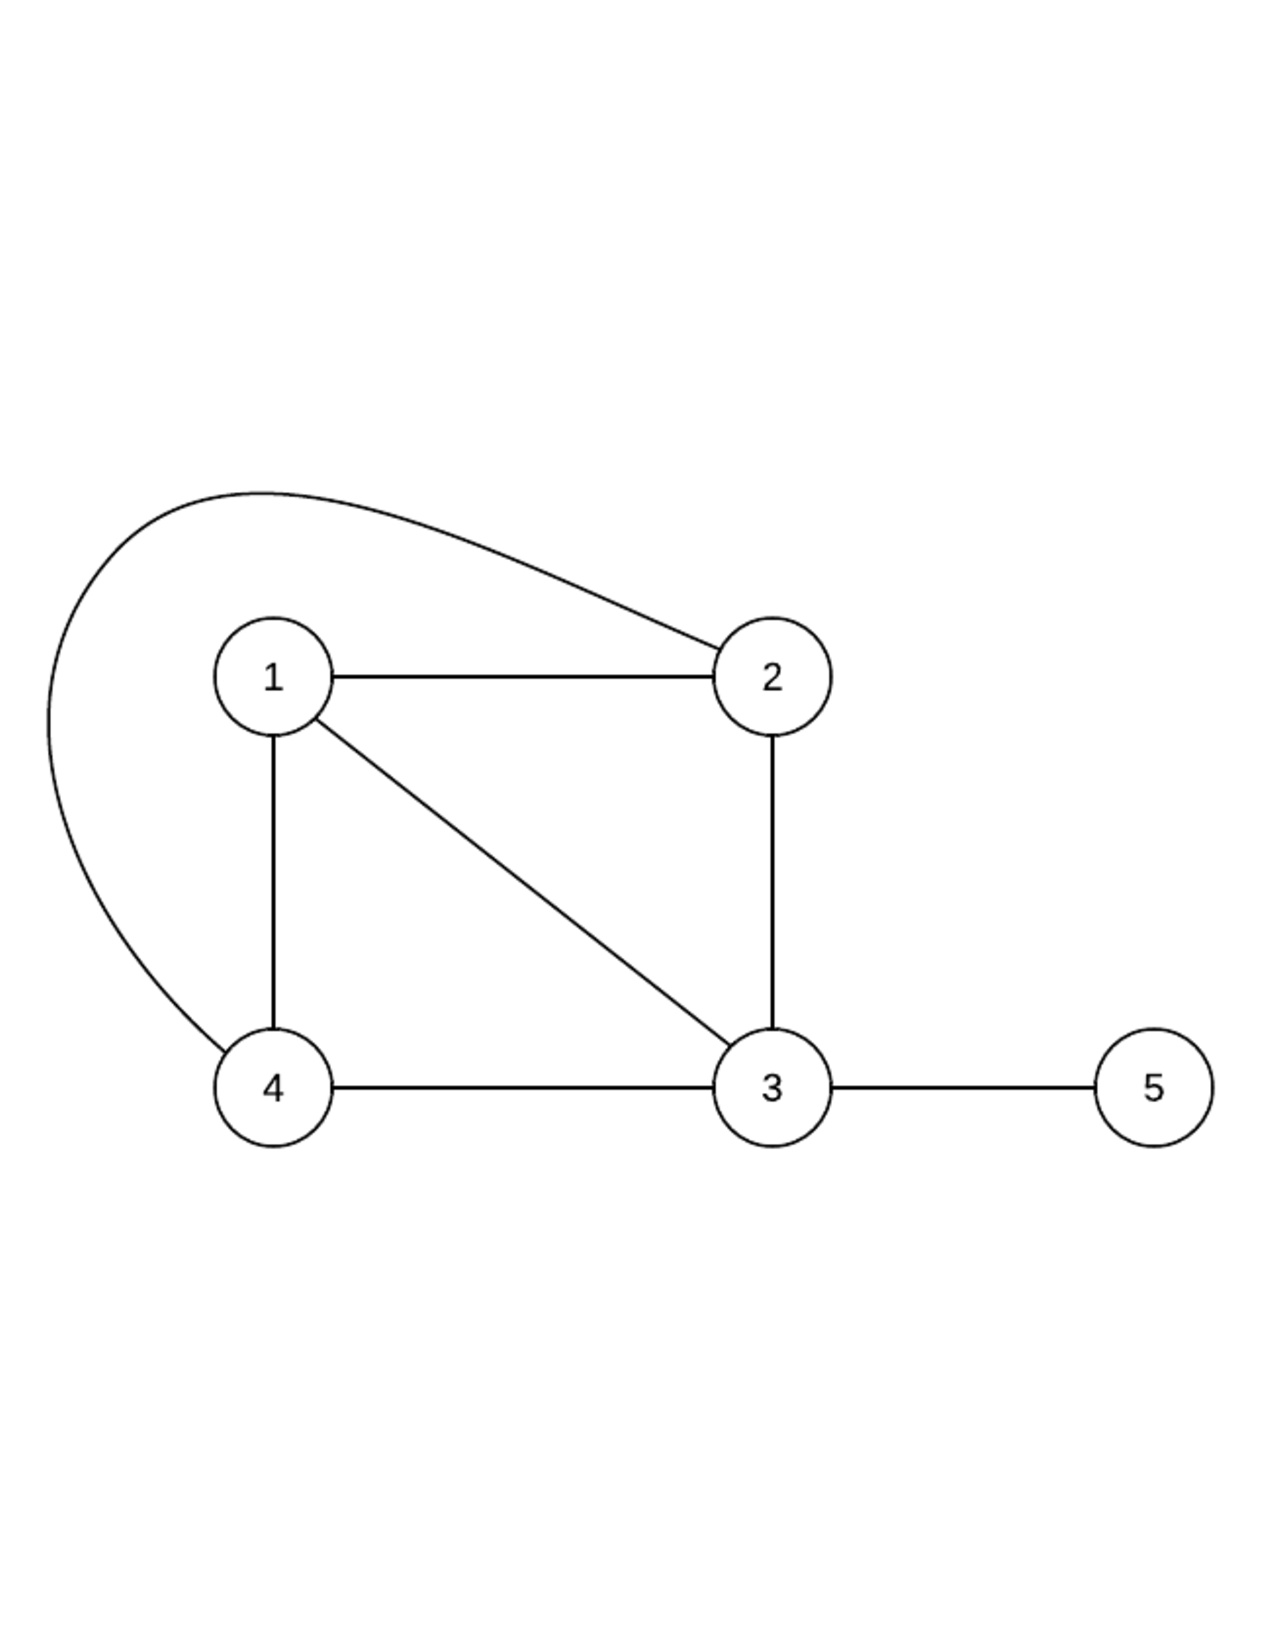
\includegraphics[scale=0.7]{simple_graph.jpg} 
%\includegraphics[width=6in,height=7in]{mq1.jpg}
\end{center}
\caption{Simple graph $\mathcal{G}$}
\label{fig:simple_graph}
\end{figure}

We construct a directed graph $\mathcal{G}_{dir}$ from the simple graph $\mathcal{G}$ by choosing the direction of  each directed edge. Each edge is, independentally, equally likely to be assigned either direction. We define the events $T_1, T_2, T_3$ and $T_4$ as below.\\
$T_1$: cycle $\{1,2,3\}$ forms a directed cycle.\\
$T_2$: cycle $\{1,3,4\}$ forms a directed cycle.\\
$T_3$: cycle $\{1,2,4\}$ forms a directed cycle.\\
$T_4$: cycle $\{2,3,4\}$ forms a directed cycle.\\

\ppart Find $\pr{T_1},\; \pr{T_2},\; \pr{T_3},\; \pr{T_4}$.

\begin{solution}
$\pr{T_1}= \pr{T_2}=\pr{T_3}= \pr{T_4} = \frac{2}{2^3} = \frac{1}{4}$.\end{solution}

\ppart Find the probability that $\mathcal{G}_{dir}$ is a DAG (directed acyclic graph).

\begin{solution}
Using Inclusion-Exclusion principle,
\begin{align*}
\pr{\mathcal{G}_{dir} \; is \; DAG} &= 1 - \pr{T_1 \cup T_3 \cup T_3 \cup T_4}\\
&= 1 - \displaystyle\sum_{i=1}^{4}\pr{T_i} + \displaystyle\sum_{i\neq j}\pr{T_i \cap T_j} - \displaystyle\sum_{i\neq j \neq k}\pr{T_i \cap T_j \cap T_k} + \pr{T_1 \cap T_2 \cap T_3 \cap T_4}\\
&=1 - 4 \cdot \frac{1}{4} + 6 \cdot \frac{1}{16} - 0+ 0\\
&= \frac{3}{8}
\end{align*}

Observe that,\\
 $\pr{T_i \cap T_j}= \frac{2}{2^5}$ for $i \neq j$,\\
 $\pr{T_i \cap T_j \cap T_k} =0$ for $i \neq j \neq k$, and\\
 $\pr{T_1 \cap T_2 \cap T_3 \cap T_4}=0$.
\end{solution}

\ppart Find the minimum DAG with the same postive walk relation as the DAG in Figure ~\ref{fig:directed_graph}.

\begin{figure}[here]
\begin{center}
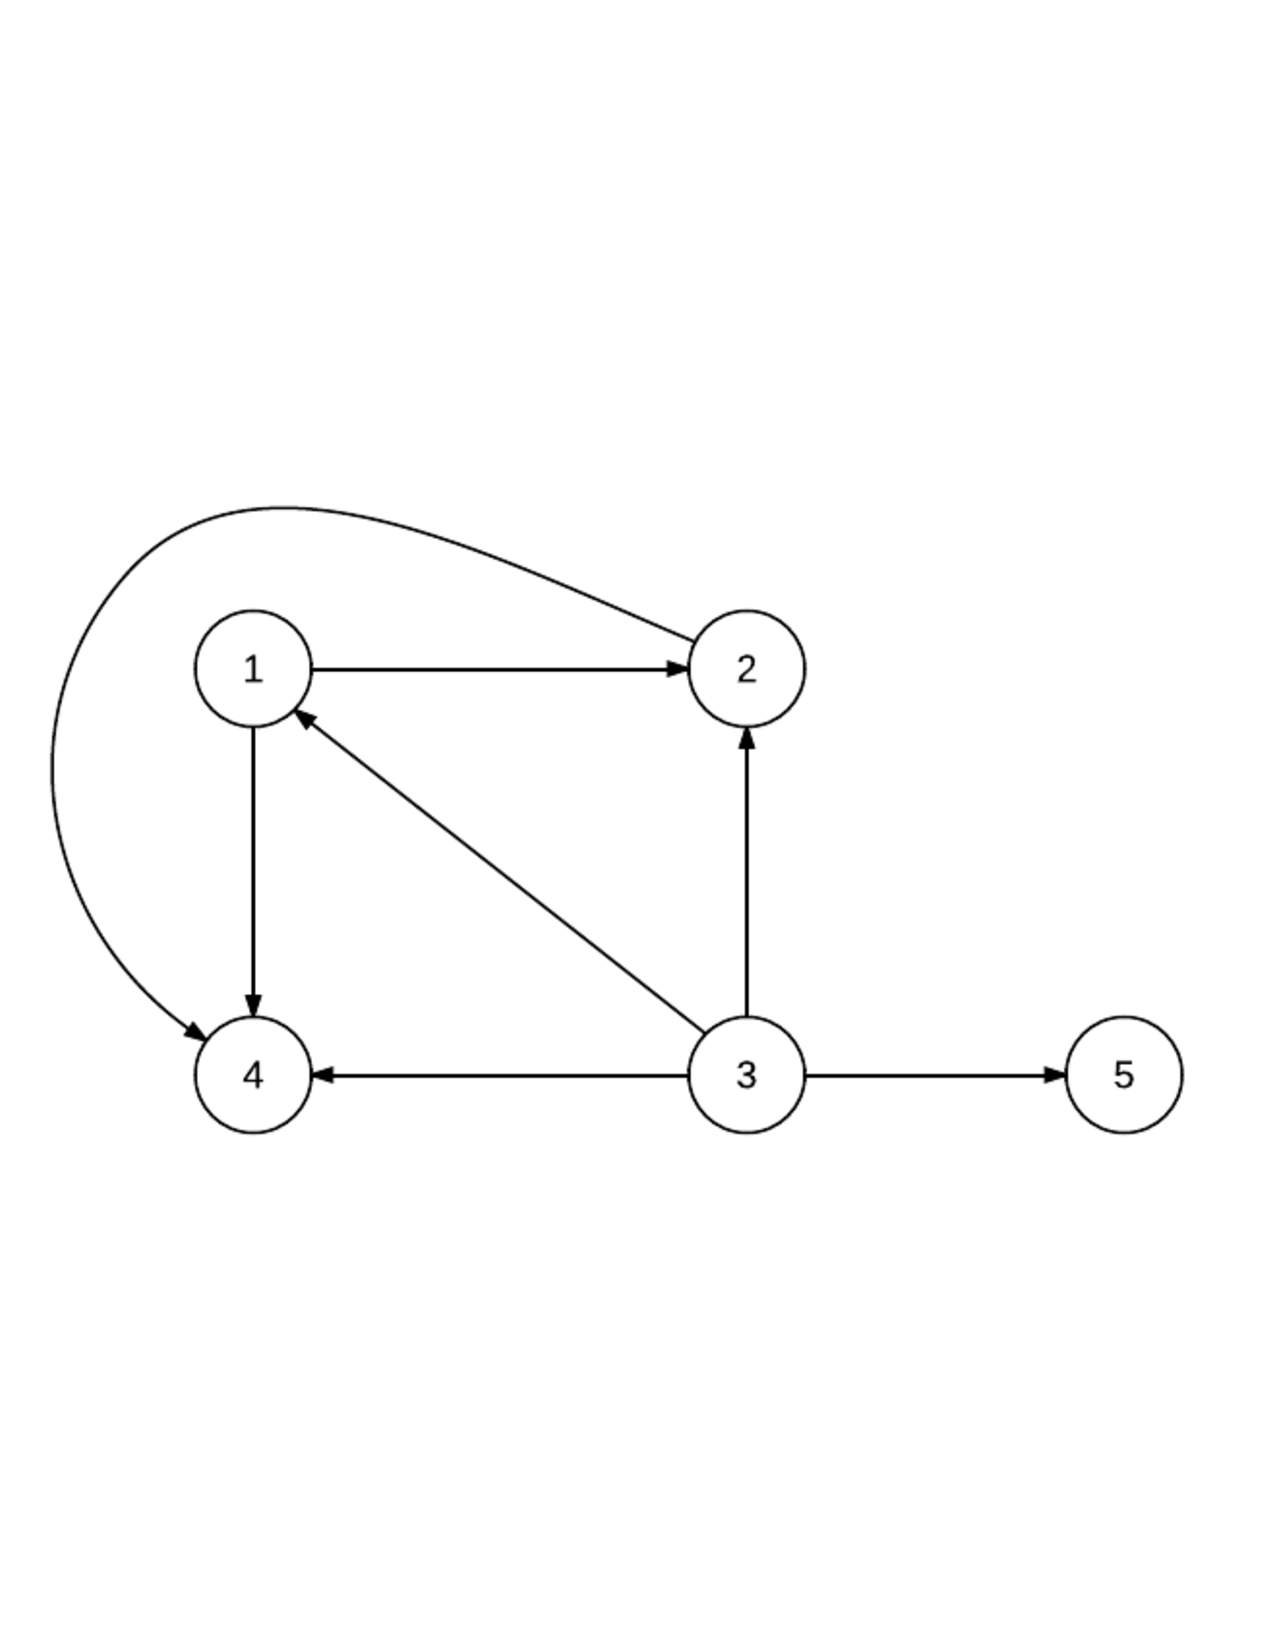
\includegraphics[scale=0.7]{dir_graph.png} 
%\includegraphics[width=6in,height=7in]{mq1.jpg}
\end{center}
\caption{DAG}
\label{fig:directed_graph}
\end{figure}

\begin{solution}
After removing edges $\diredge{3}{2}$ and $\diredge{3}{4}$, we get the minimum DAG.
\end{solution}

\ppart Find a maximal antichain for the DAG in Figure ~\ref{fig:directed_graph}.

\begin{solution}
There are multiple maximal antichains. $\{1,5\}$, $\{2,5\}$, $\{4,5\}$, etc.
\end{solution}

\eparts

\end{problem}

%%%%%%%%%%%%%%%%%%%%%%%%%%%%%%%%%%%%%%%%%%%%%%%%%%%%%%%%%%%%%%%%%%%%%
% Problem ends here
%%%%%%%%%%%%%%%%%%%%%%%%%%%%%%%%%%%%%%%%%%%%%%%%%%%%%%%%%%%%%%%%%%%%%

\endinput
